\section{Build and Deployment Design}
\subsection{Project structure and build}
The source code is kept in the folder \texttt{exam-scheduler/} of the team repository. The packages of Section~2.2 are under \texttt{src/main/java/com/team2/examscheduler}, the help text under \texttt{src/main/resources}, the tests under \texttt{src/test/java} and the sample CSV files under \texttt{sampleData}. The code is compiled with a Java Development Kit against the JavaFX libraries and packed into one file, \texttt{exam-scheduler.jar}, whose entry point is the class \texttt{Main}. Started without arguments, \texttt{Main} opens the JavaFX main window; started with the arguments \texttt{-{}-classrooms}, \texttt{-{}-registrations}, \texttt{-{}-days} and \texttt{-{}-slots}, it generates a schedule from the given files without a window and prints it, which is used for automated tests.

\subsection{Packaging and installation}
Non-functional Requirement~2 allows only a Java Runtime Environment on the user's computer, but JavaFX is not part of a standard Java Runtime Environment. Therefore the application will be delivered as a Windows installer that contains its own runtime: the \texttt{jpackage} tool of the JDK builds a reduced Java runtime that includes only the modules the application needs (the Java base modules and \texttt{javafx.controls} and \texttt{javafx.web}) and packs it together with \texttt{exam-scheduler.jar} into \texttt{ExamScheduler-1.0.exe}. The installer lets the user choose the installation folder and creates a Start menu entry and a desktop shortcut. After installation the folder \texttt{ExamScheduler} contains \texttt{app/exam-scheduler.jar} and \texttt{runtime/}; the user does not have to install Java or JavaFX. The application uses no database and no network: all data is read from the CSV files that the user selects and is kept in memory.

\subsection{Automated build}
\begin{figure}[H]\centering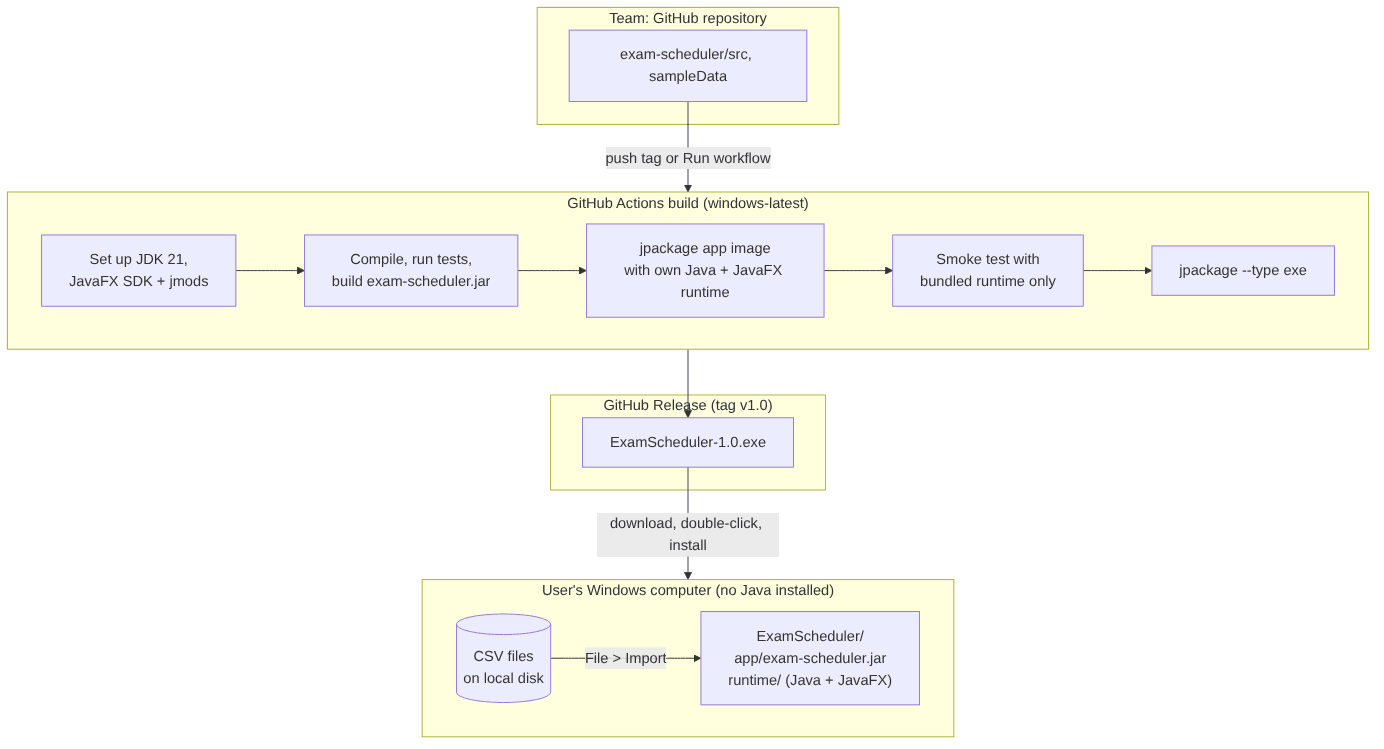
\includegraphics[width=\textwidth]{figures/deployment.png}\caption{Building, releasing and installing the Exam Scheduler.}\end{figure}
The installer will be built by a GitHub Actions workflow on a Windows machine, so that every build uses the same tools. The workflow will be started by hand or by pushing a version tag such as \texttt{v1.0}. It sets up JDK~21 and the JavaFX SDK, compiles the code, runs the tests on the sample data, builds the jar file, creates the application image with the bundled runtime and runs a smoke test that uses only this runtime, and finally builds the installer. For a version tag the installer will be attached to the GitHub Release of that version, from where the user downloads it.

\subsection{Installer test}
Before the release the installer will be tested on a Windows computer without Java, JavaFX or development tools: the installer is run, the application is started from the Start menu, the two sample files are imported, a schedule is generated for 10 days with 4 slots per day, the help is opened and the four views are checked. Problems found in this test will be recorded in GitHub Issues.
